\chapter{Iteration 1: Design and Implementation}\label{ch:iter1}

\section{Iteration Objectives}
Deliver a working vertical slice on real data: a technician selects a real aircraft, reads its dated records, enters a symptom, receives a ranked, evidence-linked investigation, opens a cited record, and sees a real correction or conflict. The same commit has automated tests and a continuous-integration run, and every failure path is reported honestly.

\section{Selected Use Cases / Features}
UC-03 (view history), UC-04 (upload report), UC-05 (start diagnosis), UC-06 (ask follow-up), UC-07 (inspect evidence), UC-08 (review conflict) and UC-09 (explore graph), as defined in Chapter~\ref{ch:req}.

\section{Design}
The design is in Chapter~\ref{ch:design}. Three iteration-specific design rules governed the work:
\begin{enumerate}
\item \textbf{The interface reflects the backend and never improves on it.} It may add labels and warnings; it may not hide, alter or invent a value.
\item \textbf{Real data or a stated reason.} A missing live model or graph is reported, never replaced by a stub that looks like a result.
\item \textbf{One owner per file, contracts frozen.} The diagnose request and response were fixed early so that three people could build in parallel.
\end{enumerate}

\section{Implementation}\label{sec:setup}
\subsection{Reproducing the system}
The full guide is \code{docs/mid1_setup.md}. In outline, with Docker, Python 3.11 and Node 20:
\begin{lstlisting}
# 1. Graph database
docker compose up -d neo4j
# 2. Backend (environment values, never committed, go in backend/.env)
cd backend && python -m venv venv && . venv/bin/activate
pip install -r requirements.txt
python scripts/fetch_sdr_data.py          # downloads the FAA 2025 file, builds the corpus
uvicorn main:app --port 8000               # DEMO_MODE=false, NEO4J_URI, NEO4J_PASSWORD, GROQ_API_KEY
curl -X POST localhost:8000/api/maintenance/ingest   # loads 2,079 records
# 3. Frontend
cd ../frontend && npm ci && npm run dev    # http://localhost:5173
# 4. Checks
cd ../backend && python -m pytest -q
cd ../frontend && npm test && npm run build
\end{lstlisting}
\code{GET /api/health} must report \code{graph_mode: neo4j} and a non-zero record count before any claim of ``real data'' is made. A Docker Compose smoke test in CI starts the whole stack and checks health, the corpus and the maintenance APIs. We have not yet had a person outside the team follow the guide on a clean machine (acceptance test T15).

\subsection{Repository layout}
\begin{longtable}{p{0.3\textwidth}p{0.6\textwidth}}
\toprule \textbf{Path} & \textbf{Content} \\ \midrule \endhead
\code{backend/api/routes} & HTTP routes \\
\code{backend/services} & Retrieval, ranking, citation check, conflict engine, budget, model client \\
\code{backend/agents} & Ingest agent \\
\code{backend/graph} & Schema, repository (queries), Neo4j client, in-memory store \\
\code{backend/tests} & 194 PyTest tests \\
\code{frontend/src} & Pages, components, hooks, utilities, API client; 171 Vitest tests in \code{src/test} \\
\code{knowledge/} & Context, flows, decision records \\
\code{docs/mid1/} & Dated evidence: audits, measurements, screenshots \\
\code{.github/workflows} & CI, staging deployment, log retrieval \\
\bottomrule
\end{longtable}

\section{Completed Features / Module}
\begin{description}
\item[M02 Assets.] \code{Assets} lists 118 aircraft with record counts from one aggregation query, searchable by tail number. \code{AssetHistory} shows an aircraft's records oldest first with identifiers, a ``Corrected by'' banner when a later record supersedes one, and deep links (\code{#recordId}) that scroll to and mark a record. \code{ServiceRecords} is a fleet-wide, URL-backed, paginated list with filters for text, status, analysis state, component and date.
\item[M03 Knowledge graph.] \code{Graph} loads the stored graph and shows one aircraft's subgraph: the aircraft, its records, and the edges between them. It states the true counts and draws \code{SUPERSEDES} apart from the other edges, with a legend that says where each comes from. A fallback for browsers without WebGL is in an open pull request and is not part of the commit this report cites.
\item[M04 Diagnostics.] \code{Diagnostics} has a multi-turn Copilot and a one-shot ``Quick diagnose''. Both show the ranked checks, the evidence records (each a link), the model's explanation when one exists, and the citation status.
\item[M05 Conflict intelligence.] \code{ReviewQueue} shows the incoming record beside the retrieved prior record with the label, score and rationale, and offers accept and reject. A second tab lists detected corrections with a component-change rate.
\item[M06 Report intelligence.] \code{MaintenanceIngest} uploads a CSV (explicit confirmation step, backend counts) or submits one record.
\end{description}

\section{Technical Implementation Details}
\subsection{Ingest}
\code{MaintenanceAgent} reads the CSV with every column as a string (a tail number such as \code{26226} must not become an integer). For each row it checks the tail, the date and the identifier, finds or creates the \code{Asset}, skips a record whose identifier already exists (re-asserting its \code{ABOUT} link), creates the \code{ServiceRecord} as unscored, links it to its aircraft, and links it to the previous record on that aircraft with \code{PRECEDED_BY}, in date order. It returns counts: records created, duplicates skipped, rows skipped for no tail, and rows skipped for a bad date or missing identifier.

\subsection{Retrieval and ranking}\label{sec:alg-rank}
\textbf{Context.} For a diagnosis the backend takes the aircraft's most recent records (default 30) and scans up to 2,500 records from other aircraft. Each fleet record is scored by
\[
s_{\text{fleet}} = 0.5\,[\text{JASC code equal}] + 0.3\,J(\text{symptom},\text{part name}) + 0.2\,J(\text{symptom},\text{record text}),
\]
where $J$ is the Jaccard similarity of the two word sets \citep{jaccard1912}; records scoring below 0.05 are dropped and the best 20 are kept.

\textbf{Ranking.} Each component (part name) receives the sum of its evidence weights:
\[
\text{score}(c) = \sum_{i\in H_c} \frac{0.4}{i+1}\,p_i \;+\; \sum_{r\in F_c} 0.6\, s_{\text{fleet}}(r)\, p_r ,
\qquad p = \begin{cases}0.3 & \text{record superseded}\\ 1 & \text{otherwise}\end{cases}
\]
with $H_c$ the aircraft's own recent records for component $c$ (position $i$ counted from the newest, starting at 0) and $F_c$ the fleet matches. Ties are broken by evidence count (higher first), then by component name, so the order is the same on every run. The weights (0.4, 0.6, 0.3) are constants chosen by the team and are not fitted to data; the score is a ranking aid, not a probability, and the interface says so.

\textbf{Copilot.} The Copilot repeats retrieval over all symptoms and observations the user has accumulated, excludes components the user has ruled out, excludes superseded records from recommendations (they stay visible as evidence), and reports which checks moved up, moved down, appeared or dropped since the previous turn.

\subsection{Citation validation}
Every token shaped like an FAA identifier (two to six capital letters followed by at least six digits) in the model's text is looked up in the graph. Those found are \code{valid}; the rest are \code{invalid} and are wrapped as \code{[UNVERIFIED:id]} in the displayed text. This confirms that a record exists; it does not confirm that the sentence citing it is supported, and the interface says that too.

\subsection{Conflict engine}
\textbf{Candidates.} For a record $r$ on aircraft $a$, every earlier record on $a$ is scored: \code{same part name} +3, \code{same JASC code} +2, \code{same location} +1, \code{within 30 days} +1. Only records with a positive score are candidates; ties are ordered by date (newest first) and identifier; at most 25 are kept. Records from the future are never compared, which prevents leakage.

\textbf{Classification.} The model returns a label (\code{no_conflict}, \code{scope_disjoint}, \code{supersedes}, \code{partial_supersedes}, \code{contradicts}) and a one-sentence rationale for the top candidate. An unparseable reply is flagged and routed to review.

\textbf{Confidence.} Signals are summed with weights that depend on whether the new record contains the FAA phrase ``SUPPLEMENTAL REPORT FOR'':
\begin{center}
\begin{tabular}{lcc}
\toprule \textbf{Signal} & \textbf{With phrase} & \textbf{Without} \\ \midrule
Explicit supersession language & 0.40 & 0 \\
Model says supersedes / partially & 0.20 & 0.35 \\
New record is clearly later & 0.15 & 0.25 \\
Source authority not lower & 0.10 & 0.15 \\
Same part and JASC code & 0.10 & 0.15 \\
Within 30 days & 0.05 & 0.10 \\
\bottomrule
\end{tabular}
\end{center}
The result is clamped to $[0,1]$. In cascade mode the model signal is scaled by vote agreement.

\textbf{Routing.} An unparseable reply, \code{contradicts} and \code{partial_supersedes} always go to review; \code{no_conflict} and \code{scope_disjoint} need no action; \code{supersedes} is accepted automatically only when confidence reaches the threshold 0.50, which the earlier evaluation selected and which we did not change to improve a demonstration. Only an accepted supersession creates a \code{SUPERSEDES} edge and marks the older record superseded.

\subsection{Honest analysis state and the cost cascade}
Ingest never invents a score: records start unscored with a null confidence. Analysis runs separately (a command-line resume, or a batch endpoint limited to 25 records and protected by an operations token), needs a live model, and stops cleanly at 90\% of a per-day request or token budget. Records ingested by an early version that carry an untouched confidence of 1.0 are reported by the API as unscored instead of as a perfect score.

The cascade is off by default and was pre-registered before it was evaluated. A deterministic text and scope screen (threshold 0.79) removes pairs that need no model request; for the rest, two votes are taken and escalated to five only on disagreement; a persistent split goes to review. Method, model, votes, passes and token use are stored with every result.

\subsection{Frontend technical decisions}
\begin{itemize}
\item \textbf{One failure model.} A single helper turns a failed request into a plain message (unreachable, not found, service unavailable, server error), so no page shows an empty state when the real cause is a failure.
\item \textbf{Selection, never invention.} The graph page only \emph{selects} nodes and edges the backend stored (one aircraft, maintenance nodes only); it never creates an edge.
\item \textbf{Server-confirmed actions.} Accept and reject update the screen only after a successful response; buttons lock while a request is pending.
\item \textbf{Two-step upload.} Choosing a CSV changes nothing; ingesting is a separate confirmed action because it writes to the graph.
\end{itemize}

\section{Algorithms and Technical Decisions}
The algorithms are described in the subsections above; the reasons for the main choices are in Table~\ref{tab:findings} and Table~\ref{tab:dec}. Two limits matter for how the results may be read. The ranking weights are not tuned and have not been evaluated against baselines. The confidence threshold was selected on an earlier evaluation with a different model from the one now configured on staging.

\section{Tools, Frameworks and Technologies}\label{sec:external}
\begin{longtable}{p{0.27\textwidth}p{0.2\textwidth}p{0.45\textwidth}}
\caption{External components and tools}\label{tab:tools}\\
\toprule \textbf{Component} & \textbf{Version} & \textbf{Purpose} \\ \midrule \endfirsthead
\toprule \textbf{Component} & \textbf{Version} & \textbf{Purpose} \\ \midrule \endhead
FastAPI, Uvicorn & 0.111.0, 0.30.1 & Backend web framework and server \\
Pydantic Settings & 2.3.1 & Configuration and request validation \\
Neo4j (database, Python driver) & 5, 5.20.0 & Graph storage and queries \\
Groq Python client & 0.9.0 & Calls to the hosted language model \\
pandas & 2.2.2 & CSV loading and data preparation \\
PyTest, pytest-cov & 8.2.2, 5.0.0 & Backend tests \\
React, React Router & 18.3, 6.24 & Frontend framework and routing \\
Vite, Tailwind CSS & 5.3, 3.4 & Build tool and styling \\
Axios & 1.7 & HTTP client \\
\code{react-force-graph-3d}, three & 1.24, 0.185 & Interactive 3D graph \\
Vitest, Testing Library, jsdom & 2.1, 16, 29 & Frontend tests \\
Docker Compose & v2 & Local and CI full-stack runs \\
GitHub Actions & --- & CI and staging deployment \\
Vercel & --- & Frontend hosting and previews \\
Groq-hosted model & \code{openai/gpt-oss-120b} (evaluation) and \code{openai/gpt-oss-20b} (current default) & Phrasing and classification; replaceable \\
\bottomrule
\end{longtable}
The model is an external component. Replacing it changes classification quality but not the ranking, the graph, the citation check or the review workflow.

\section{Demonstration Evidence}\label{sec:demo}
The figures below are screenshots of the running application. Figures~\ref{fig:shot-assets} to~\ref{fig:shot-fail} were captured on 16 October against a local stack holding the full corpus with a live model. Figures~\ref{fig:shot-records} to~\ref{fig:shot-ingest} were captured on 18 October against a local scratch graph that holds only aircraft 800NN, which was analysed for this purpose (Section~\ref{sec:oneaircraft}); they are not staging.

\begin{figure}[H]\centering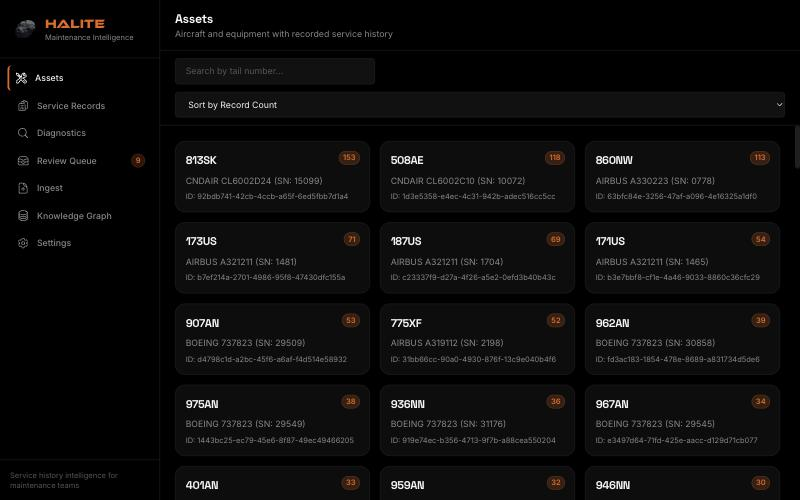
\includegraphics[width=0.92\textwidth]{02_assets_live_corpus.jpg}\caption{Assets: the real corpus with record counts.}\label{fig:shot-assets}\end{figure}
\begin{figure}[H]\centering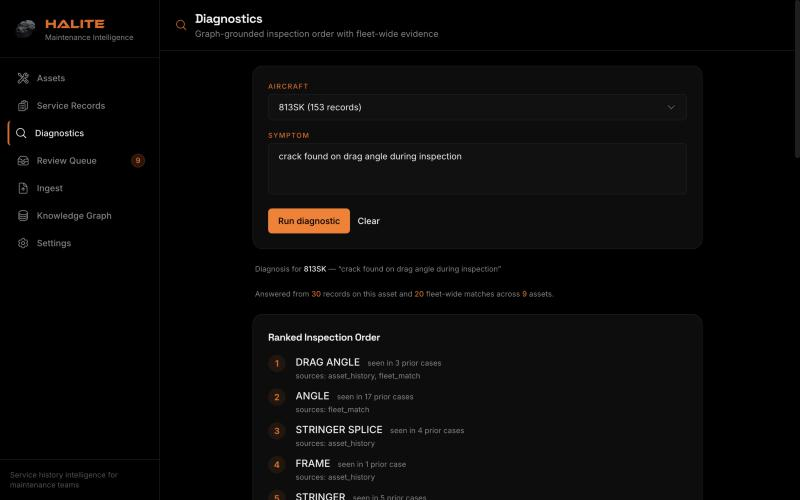
\includegraphics[width=0.92\textwidth]{06_diagnostics_ranked_checks.jpg}\caption{Quick diagnose for aircraft 813SK: ranked inspection order with sources.}\label{fig:shot-diag}\end{figure}
\begin{figure}[H]\centering
\includegraphics[width=0.92\textwidth]{07_diagnostics_analysis_citations_evidence.jpg}\caption{The model's explanation, the line ``12 cited record IDs verified against the graph'', and the evidence records, each a link.}\label{fig:shot-cite}\end{figure}
\begin{figure}[H]\centering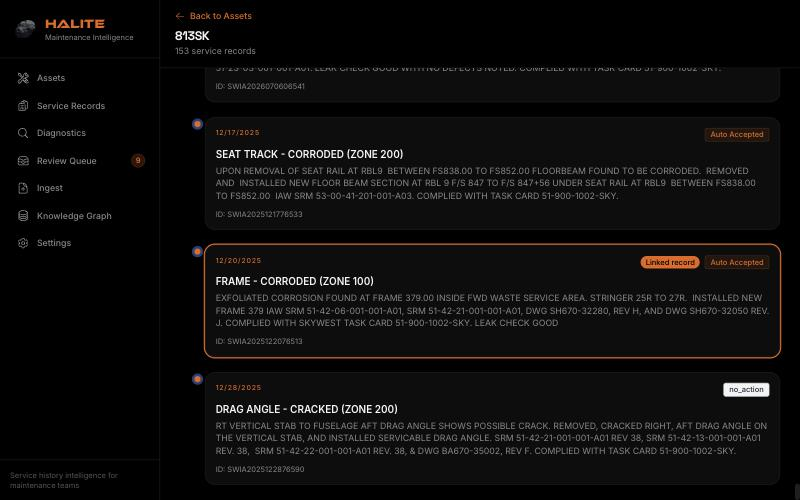
\includegraphics[width=0.92\textwidth]{03_history_linked_record.jpg}\caption{Asset History opened on a cited record, marked as the linked record.}\label{fig:shot-history-linked}\end{figure}
\begin{figure}[H]\centering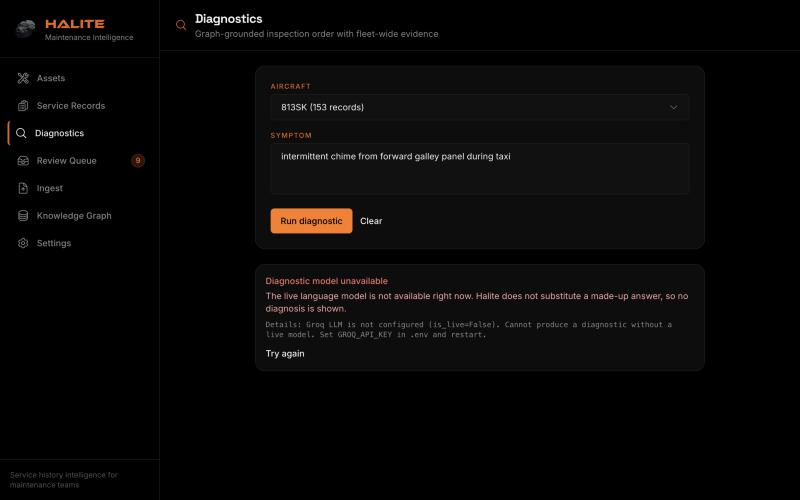
\includegraphics[width=0.92\textwidth]{10_diagnostics_model_unavailable_real_503.jpg}\caption{Failure case: the model is unavailable. The backend's real HTTP 503 reason is shown and no diagnosis is invented.}\label{fig:shot-fail}\end{figure}
\begin{figure}[H]\centering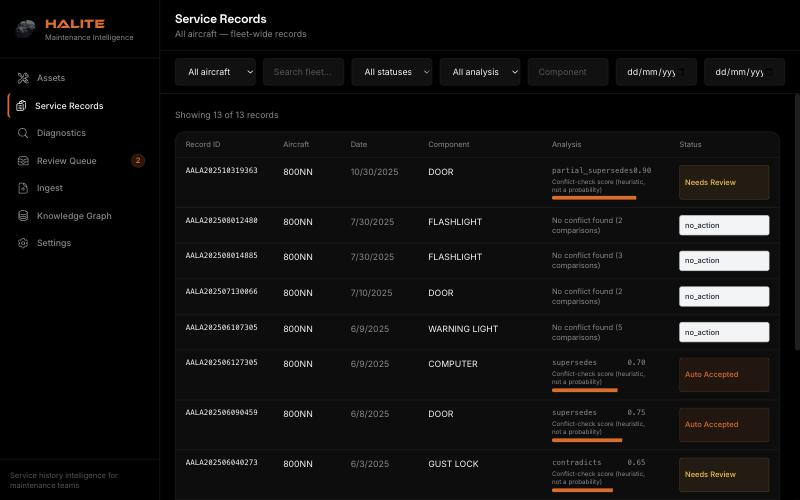
\includegraphics[width=0.92\textwidth]{14_records_scored_800NN.jpg}\caption{Service Records for aircraft 800NN after analysis: label, score (marked heuristic, not a probability) and status per record.}\label{fig:shot-records}\end{figure}
\begin{figure}[H]\centering
\includegraphics[width=0.92\textwidth]{15_history_correction_800NN.jpg}\caption{Asset History: the older DOOR TRACK record is greyed and reads ``Corrected by \ldots component changed DOOR TRACK $\to$ DOOR''.}\label{fig:shot-history}\end{figure}
\begin{figure}[H]\centering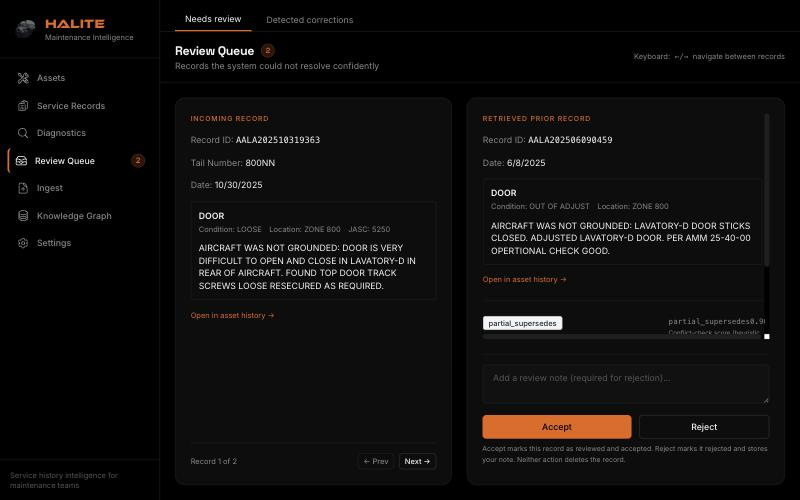
\includegraphics[width=0.92\textwidth]{16_review_queue_800NN.jpg}\caption{Review Queue: the incoming record beside the retrieved prior record, with the model's rationale and the accept and reject actions (not used on this data).}\label{fig:shot-review}\end{figure}
\begin{figure}[H]\centering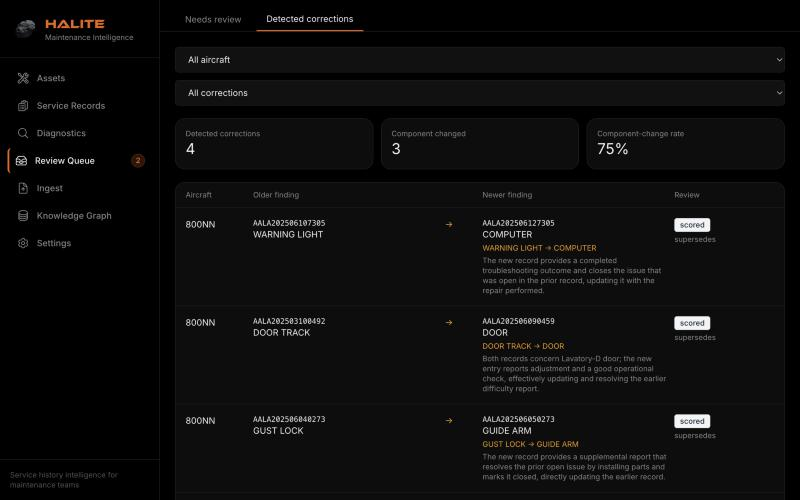
\includegraphics[width=0.92\textwidth]{17_corrections_tab_800NN.jpg}\caption{Detected corrections: four found, three with a component change.}\label{fig:shot-corr}\end{figure}
\begin{figure}[H]\centering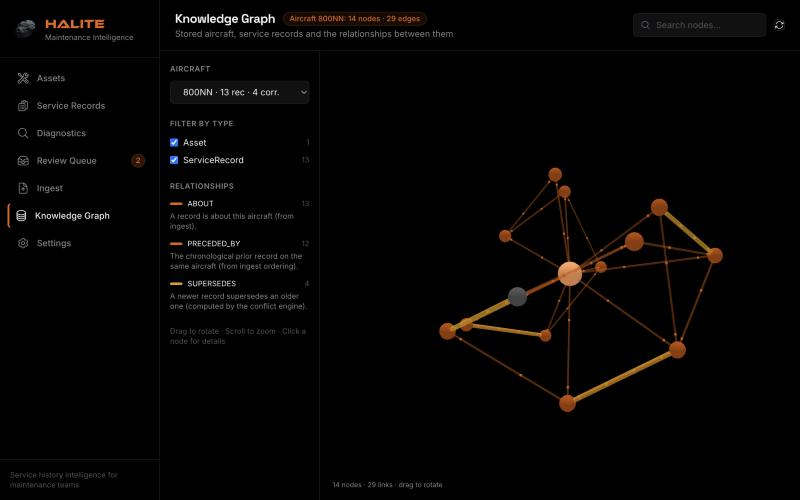
\includegraphics[width=0.92\textwidth]{18_graph_800NN_amber_corrections.jpg}\caption{Knowledge Graph for aircraft 800NN: 14 nodes and 29 edges; the four \code{SUPERSEDES} corrections are thick and amber, the superseded record is grey.}\label{fig:shot-graph}\end{figure}
\begin{figure}[H]\centering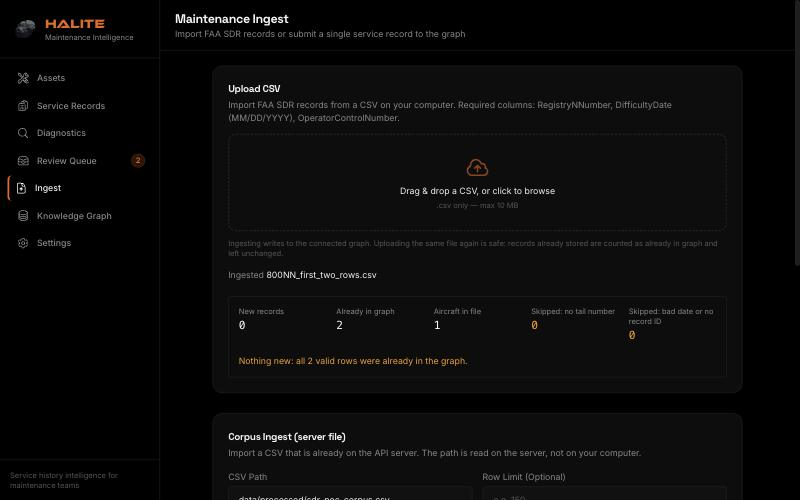
\includegraphics[width=0.92\textwidth]{19_ingest_upload_nothing_new.jpg}\caption{Ingest: re-uploading rows that are already stored reports zero new records and the duplicates, and changes nothing.}\label{fig:shot-ingest}\end{figure}

\section{Iteration Outcome}
Every feature planned for the iteration is implemented at the level stated in Table~\ref{tab:progress}, with three qualifications: retrieval is lexical, the ranking is a heuristic that has not been evaluated against baselines, and the full corpus has not been analysed. The slice runs on real data, is covered by automated tests, and reports its own failures.
